% Meta-ORES entities and their relationships.
\documentclass{article}
\usepackage{tikz}
\usetikzlibrary{arrows,shapes}

\begin{document}
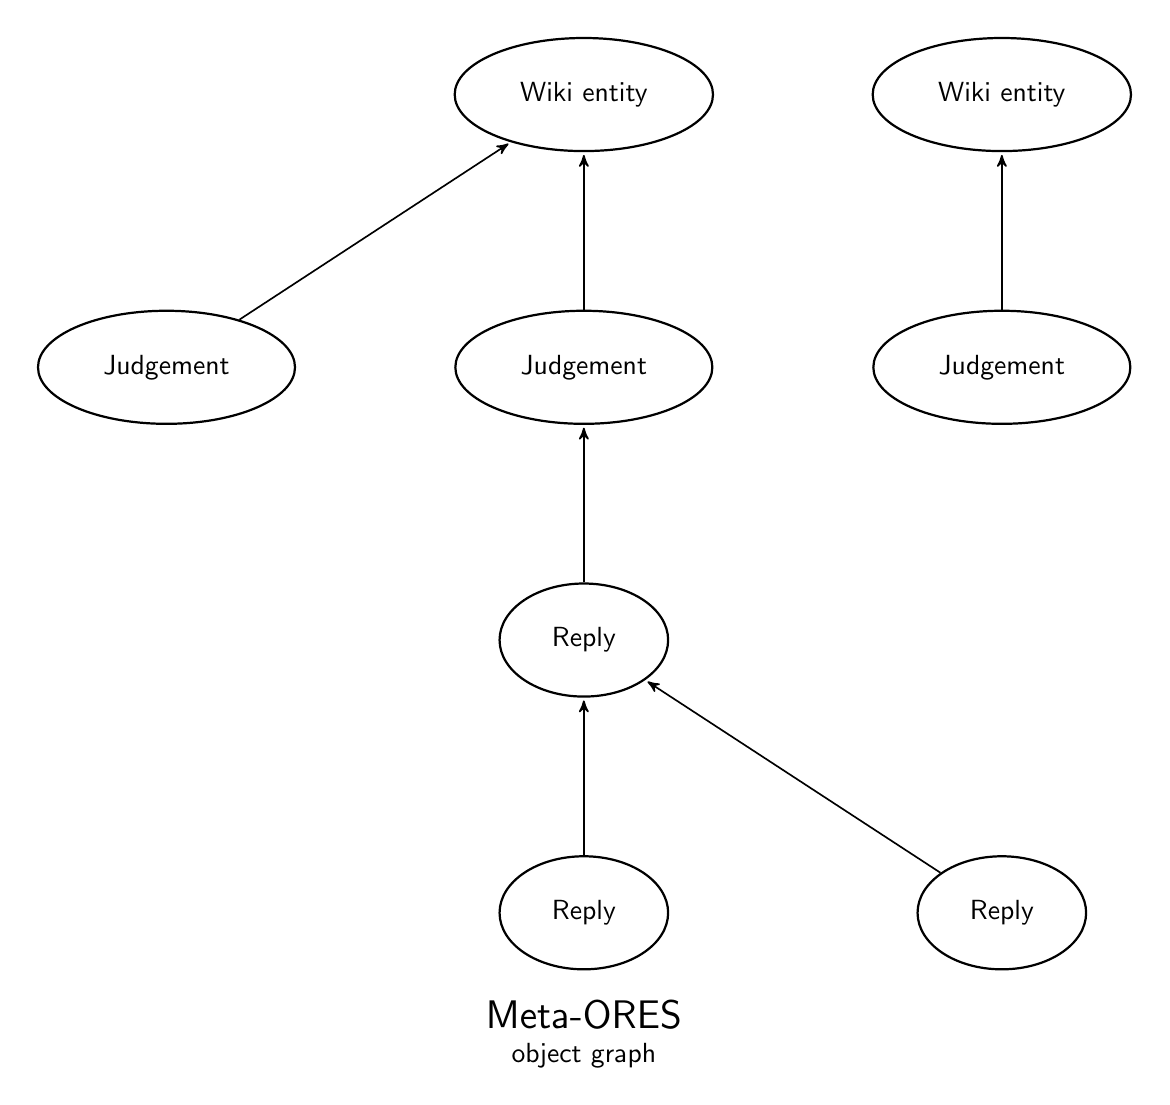
\begin{tikzpicture}[
  font=\sffamily,
  every matrix/.style={ampersand replacement=\&, column sep=2cm, row sep=2cm},
  entity/.style={draw, ellipse, thick, inner sep=1em},
  owned/.style={->, >=stealth', shorten >=1pt, semithick, font=\sffamily\footnotesize},
  every node/.style={align=center}]

  % TODO: dashed boxes for regions: wiki entity, judgement, discussion

  % Position the nodes using a matrix layout
  \matrix{
        \& \node[entity] (wiki1) {Wiki entity};
			\& \node[entity] (wiki2) {Wiki entity}; \\
	  % FIXME: Vary node styles?
      \node[entity] (comment1) {Judgement};
		\& \node[entity] (comment2) {Judgement};
			\& \node[entity] (comment3) {Judgement}; \\
		  \& \node[entity] (reply1) {Reply}; \\
		  \& \node[entity] (reply2a) {Reply};
		  \& \node[entity] (reply2b) {Reply}; \\
  };

  \node [below=1cm, align=flush center] at (reply2a)
  {\Large Meta-ORES \\ \normalsize object graph};

  % Draw the arrows between the nodes and label them.
  \draw[owned] (comment1) -- (wiki1);
  \draw[owned] (comment2) -- (wiki1);
  \draw[owned] (comment3) -- (wiki2);
  \draw[owned] (reply1) -- (comment2);
  \draw[owned] (reply2a) -- (reply1);
  \draw[owned] (reply2b) -- (reply1);
\end{tikzpicture}
\end{document}
